
%(BEGIN_QUESTION)
% Copyright 2007, Tony R. Kuphaldt, released under the Creative Commons Attribution License (v 1.0)
% This means you may do almost anything with this work of mine, so long as you give me proper credit

If the gain, lag time, and dead time of a process are known, it is possible to program a computer to mimic these dynamic elements in mathematical form.  Such a program is called a {\it model} of the process.

Models can be very helpful for advanced control strategies.  Take for instance this strategy, known as the {\it Smith Predictor}: its purpose is to ``cancel out'' dead time in a process control loop, so that setpoint changes may be made without overshoot or long response lags.

$$\includegraphics[width=15.5cm]{i01775x01.eps}$$

Explain how the Smith Predictor strategy would respond to a sudden increase in setpoint (r).

\underbar{file i01775}
%(END_QUESTION)





%(BEGIN_ANSWER)

If the setpoint ($r$) increases, the PID control block will output an increased manipulated variable signal ($m$).  This increased controller output will affect the process, (eventually) increasing the process variable ($c$).  The model, internal to the controller, also responds to the increased PID output.  The gain and lag time portions of the controller's model respond immediately to the change in output, feeding back that information to the error summer so that the PID block may begin to control a ``virtual'' representation of the process without any dead time.  Meanwhile, the process response delayed by dead time is still propagating through the dead time block of the model, and the dead time of the real process.

When the response finally propagates through the dead time of process and model, the result should be the same (if the model is accurate).  These equal changes in process response cancel each other out at the subtraction block at the far right of the diagram, so that all the PID block ``sees'' is the gain and lag time of the process.

%(END_ANSWER)





%(BEGIN_NOTES)

In essence, the Smith Predictor strategy allows a PID controller to control an idealized process model (without dead time), while canceling out the dead time of the real process.  The only aspect of process dead time that a Smith Predictor does not cancel out is that caused by changes in process load.  Smith Predictor strategies eliminate dead time only in regard to changes in setpoint.

In order to completely eliminate dead time from a control loop, the Smith Predictor strategy would have to be ``aware'' of all process loads, in a feedforward scheme like this:

$$\includegraphics[width=15.5cm]{i01775x02.eps}$$

%INDEX% Control, strategies: Smith predictor
%INDEX% Documentation, block diagram: control strategy

%(END_NOTES)


